\documentclass[12pt]{article}\usepackage[]{graphicx}\usepackage[]{color}
% maxwidth is the original width if it is less than linewidth
% otherwise use linewidth (to make sure the graphics do not exceed the margin)
\makeatletter
\def\maxwidth{ %
  \ifdim\Gin@nat@width>\linewidth
    \linewidth
  \else
    \Gin@nat@width
  \fi
}
\makeatother

\definecolor{fgcolor}{rgb}{0.345, 0.345, 0.345}
\newcommand{\hlnum}[1]{\textcolor[rgb]{0.686,0.059,0.569}{#1}}%
\newcommand{\hlstr}[1]{\textcolor[rgb]{0.192,0.494,0.8}{#1}}%
\newcommand{\hlcom}[1]{\textcolor[rgb]{0.678,0.584,0.686}{\textit{#1}}}%
\newcommand{\hlopt}[1]{\textcolor[rgb]{0,0,0}{#1}}%
\newcommand{\hlstd}[1]{\textcolor[rgb]{0.345,0.345,0.345}{#1}}%
\newcommand{\hlkwa}[1]{\textcolor[rgb]{0.161,0.373,0.58}{\textbf{#1}}}%
\newcommand{\hlkwb}[1]{\textcolor[rgb]{0.69,0.353,0.396}{#1}}%
\newcommand{\hlkwc}[1]{\textcolor[rgb]{0.333,0.667,0.333}{#1}}%
\newcommand{\hlkwd}[1]{\textcolor[rgb]{0.737,0.353,0.396}{\textbf{#1}}}%
\let\hlipl\hlkwb

\usepackage{framed}
\makeatletter
\newenvironment{kframe}{%
 \def\at@end@of@kframe{}%
 \ifinner\ifhmode%
  \def\at@end@of@kframe{\end{minipage}}%
  \begin{minipage}{\columnwidth}%
 \fi\fi%
 \def\FrameCommand##1{\hskip\@totalleftmargin \hskip-\fboxsep
 \colorbox{shadecolor}{##1}\hskip-\fboxsep
     % There is no \\@totalrightmargin, so:
     \hskip-\linewidth \hskip-\@totalleftmargin \hskip\columnwidth}%
 \MakeFramed {\advance\hsize-\width
   \@totalleftmargin\z@ \linewidth\hsize
   \@setminipage}}%
 {\par\unskip\endMakeFramed%
 \at@end@of@kframe}
\makeatother

\definecolor{shadecolor}{rgb}{.97, .97, .97}
\definecolor{messagecolor}{rgb}{0, 0, 0}
\definecolor{warningcolor}{rgb}{1, 0, 1}
\definecolor{errorcolor}{rgb}{1, 0, 0}
\newenvironment{knitrout}{}{} % an empty environment to be redefined in TeX

\usepackage{alltt}
\textwidth=7in
\textheight=9.5in
\topmargin=-1in
\headheight=0in
\headsep=.5in
\hoffset  -.85in

\pagestyle{empty}

\usepackage{amsmath,amssymb,amsfonts}
\usepackage{url}

\renewcommand{\thefootnote}{\fnsymbol{footnote}}
\IfFileExists{upquote.sty}{\usepackage{upquote}}{}
\begin{document}

\begin{center}
{\bf Intro to Data Science \\ Homework 3: Due Wednesday September 25 at 2:00pm}
\end{center}

\setlength{\unitlength}{1in}

\begin{picture}(6,.1)
\put(0,0) {\line(1,0){6.5}}
\end{picture}

\renewcommand{\arraystretch}{2}

\vskip.25in

\noindent{\bf  {\Large Exercises:} }

\vskip.25in
  \begin{enumerate}
    \item   Go through section 9 Functions of the R Programming course in the {\tt swirl} package, then answer the following questions:
    \begin{enumerate}
      \item   What is a function? 
      \item What does the {\tt Sys.Data()} function do? How many input arguments are required?
      \item What are the two ``slogans'' for R stated by John Chambers? 
      \item How do you see the source code for an R function? 
      \item Why would having default arguments by useful?
      \item What does the {\tt args} function do? Give an example of its use. 
      \item Explain why one might want to pass a function as an argument to another function. 
      \item What is an easy way to return the last element of an arbitrary vector? 
      \item What does the {\tt paste} function do? 
      \item What is the significance of the ``dot-dot-dot'' argument for a function in R? 
    \end{enumerate}
    \item Write an R function that inputs a vector and computes the mean of the vector. Save your function in an R script called {\tt my\_mean\_func.R}. Be sure to test your function and make sure it is working correctly.
    \item Write an R function that inputs two whole numbers and returns the remainder after dividing the first by the second. Save your function in an R script called {\tt my\_remain\_func.R}. Be sure to test your function and make sure it is working correctly.
    \item This exercise walks you through the steps to plot the graph of a function $y=f(x)$ using the {\tt stat\_function()} function from the ggplot2 package. Here are the commands to plot $y=x^3$ over the interval $[-1,2]$:
\begin{knitrout}
\definecolor{shadecolor}{rgb}{0.969, 0.969, 0.969}\color{fgcolor}\begin{kframe}
\begin{alltt}
\hlkwd{library}\hlstd{(ggplot2)}
\hlcom{# create function for y=x^3}
\hlstd{y_cubed} \hlkwb{<-} \hlkwa{function}\hlstd{(}\hlkwc{x}\hlstd{)\{}
  \hlstd{x}\hlopt{^}\hlnum{3}
\hlstd{\}}
\hlcom{# create input values}
\hlstd{x} \hlkwb{<-} \hlkwd{seq}\hlstd{(}\hlopt{-}\hlnum{1}\hlstd{,}\hlnum{2}\hlstd{,}\hlkwc{by}\hlstd{=}\hlnum{0.05}\hlstd{)}
\hlstd{f_df} \hlkwb{<-} \hlkwd{data.frame}\hlstd{(}\hlkwc{x}\hlstd{=x)}
\hlcom{# plot graph}
\hlkwd{ggplot}\hlstd{(f_df,}\hlkwd{aes}\hlstd{(}\hlkwc{x}\hlstd{=x))} \hlopt{+} \hlkwd{stat_function}\hlstd{(}\hlkwc{fun}\hlstd{=}\hlstr{"y_cubed"}\hlstd{)}
\end{alltt}
\end{kframe}
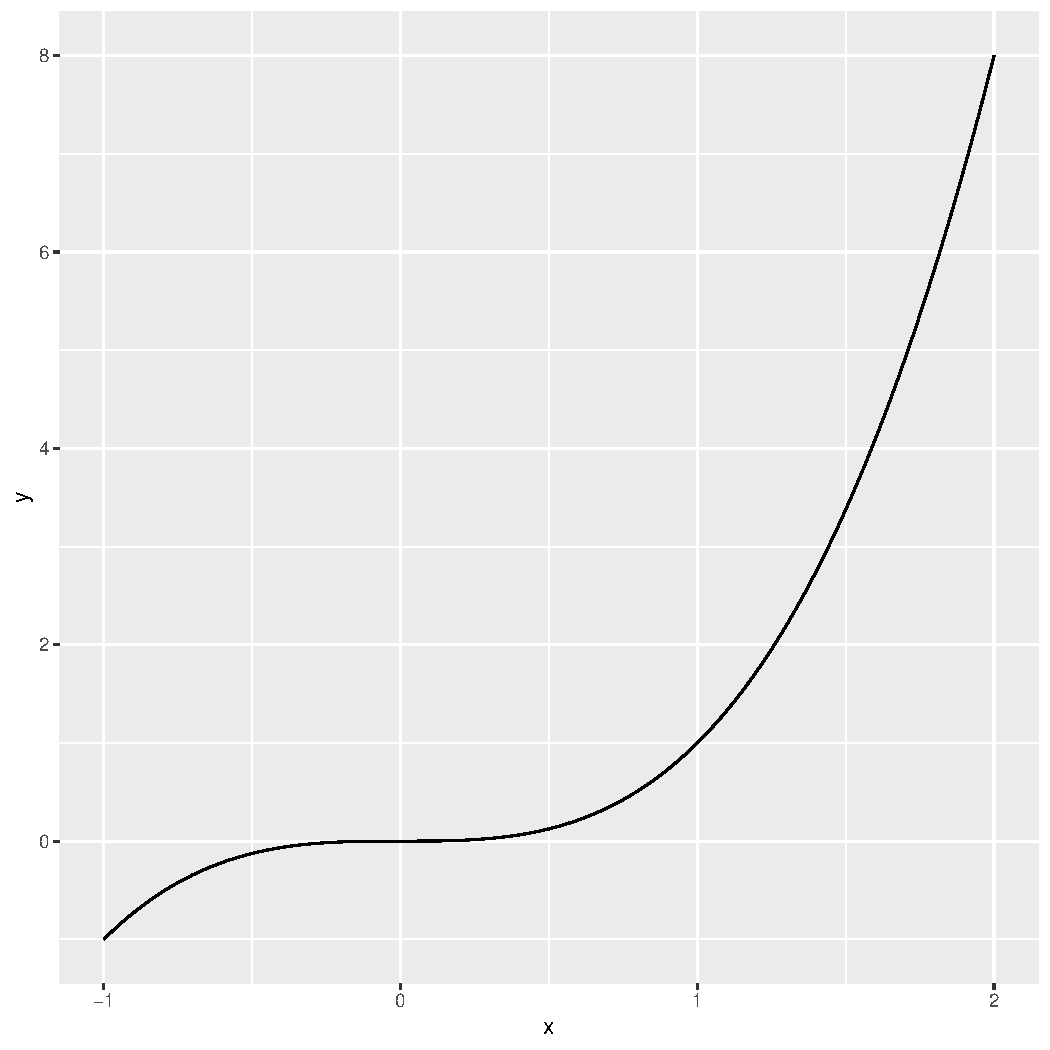
\includegraphics[width=\maxwidth]{figure/unnamed-chunk-1-1} 

\end{knitrout}
    
    \begin{enumerate}
      \item Using the previous code as a template, plot the specified functions over the given interval:
      \begin{enumerate}
        \item $y=2x^2 - 3x + 5$, $[-2,6]$
        \item $y=e^{-2x}$, $[0,3]$
        \item $y=\ln(x)$, $[0.5,3]$
      \end{enumerate}
    \end{enumerate}
    \item What trigonometric functions does R provide? Make plots of each of the trigonometric functions over an appropriate period. 
    \item Using the {\tt flights} data from the {\tt nycflights13} package,  find all flights that
    \begin{enumerate}
      \item Had an arrival delay of two or more hours
      \item Flew to Houston (IAH or HOU)
      \item Were operated by United, American, or Delta
      \item Departed in summer (July, August, and September)
      \item Arrived more than two hours late, but didn?t leave late
      \item Were delayed by at least an hour, but made up over 30 minutes in flight
      \item Departed between midnight and 6am (inclusive)
    \end{enumerate}
    \item Another useful {\tt dplyr} filtering helper is {\tt between()}. What does it do? Can you use it to simplify the code needed to answer the previous challenges?
    \item How many flights have a missing dep\_time? What other variables are missing? What might these rows represent?
    \item How could you use arrange() to sort all missing values to the start? (Hint: use is.na()).
    \item Sort {\tt flights} to find the most delayed flights. Find the flights that left earliest.
    \item Sort {\tt flights} to find the fastest flights.
    \end{enumerate}
    
\end{document}
